%!TeX root=../tese.tex
%("dica" para o editor de texto: este arquivo é parte de um documento maior)
% para saber mais: https://tex.stackexchange.com/q/78101/183146

%% ------------------------------------------------------------------------- %%
\chapter{ABB estática ótima}
\label{cap:abb-estatica-otima}

//trocar a chave $x_i$ por $i$

Neste capítulo será apresentada a solução para o problema de encontrar uma árvore binária de busca estática com custo mínimo para uma determinada sequência de acessos. O algoritmo foi desenvolvido por \cite{knuth}.

\section{Custo de uma ABB}

O custo de um acesso à chave $j$ em uma ABB estática é o número de nós acessados durante o algoritmo de busca. Como rotações não são permitidas em ABBs estáticas, a estrutura da árvore não muda, logo o custo de um acesso à chave $j$ numa tal ABB $T$ sempre é 1 mais a profundidade de $j$ em $T$. Denotaremos a profundidade do nó com chave $j$ por $d(j)$.

O custo de executar uma sequência $X = (x_{1},\ldots,x_{m})$ de $m$ acessos às chaves $1, 2,\ldots,n$ de uma ABB estática é a somatória dos custos dos acessos executados, ou seja, é
\begin{align*}
    \sum_{i=1}^{m} (d(i) + 1).
\end{align*}

Uma delimitação óbvia para este custo é que ele é no mínimo $m$, pois $d(j) \geq 0$.

Dada uma sequência $X$ de acessos, uma ABB é considerada ótima se executa os acessos de $X$ com o menor custo possível.

\section{Natureza do problema}

Definimos o custo para uma sequência de buscas em uma ABB com base em cada elemento de $X$. Porém, nota-se que é possível definir o mesmo custo com base no número de ocorrências de cada elemento desta ABB. Denotaremos por $e(j)$ o número de ocorrências de $j$ na sequência.
Cada acesso ao nó de chave $j$ contribui com $d(j) + 1$ ao custo. Como o nó com chave $j$ será acessado $e(j)$ vezes, então o nó de chave $j$ contribui com $(d(j) + 1)  \cdot e(j)$ para o custo total, ou seja,
\begin{align*}
\sum_{i=1}^{m} (d(i) + 1) &= \sum_{j=1}^{n} (d(j) + 1) \cdot e(j).
\end{align*}


Dado que a contribuição de cada chave para o custo é uma multiplicação entre a sua profundidade na ABB e seu número de ocorrências na sequência, intuitivamente é esperado que os nós mais próximos da raiz da ABB ótima guardem as chaves com os maiores números de ocorrência na sequência, já que a ABB terá que acessar esse nó múltiplas vezes. Analogamente, é esperado que os nós mais distantes da raiz da ABB ótima guardem as chaves com os menores números de ocorrência na sequência.

De maneira sucinta, é esperado que o custo de acessos mais caros, ou seja, acessos a nós mais profundos, sejam pagos menos vezes e é esperado que os custos de nós mais baratos, ou seja, acessos a nós mais superficiais, sejam pagos mais vezes.

\section{Algoritmo guloso}

É possível desenvolver um algoritmo guloso para a construção de uma ABB com base nessa intuição de priorizar que chaves com maior número de ocorrência estejam mais próximas da raiz. O Programa~\ref{prog:abb-gulosa} organiza as chaves de maneira decrescente no número de ocorrências e adiciona iterativamente à árvore um nó com a chave de maior número de ocorrências que ainda não foi adicionada. Para isso, ele utiliza uma fila de prioridades de máximo que armazenas pares ($j$, $e[j]$), considerando os vetores de $e[j]$ como chave.



% ARRUMAR O HFILL!!
% arrumar vazio
\begin{programruledcaption}{Algoritmo guloso ABB.\label{prog:abb-gulosa}}
  \noindent\textbf{Entrada}: Vetor e[1,\ldots,$n$] de ocorrências por chave e número de chaves \\
  \textbf{Saída}: ABB com as chaves 1 a $n$
  \vspace{-0.5\baselineskip}
  %função guloso_ABB(e,n)
  \begin{lstlisting}[
      language={[brazilian]pseudocode},
      style=pseudocode,
      style=wider,
      functions={},
      specialidentifiers={},
      escapeinside={(*@}{@*)},
  ]
  (*@\bfseries\scshape{Função}@*) guloso_ABB(e,n)
    Q := fila_de_prioridade() (*@ \hfill @*) // Cria uma fila de prioridade vazia
    abb := abb() (*@ \hfill @*) // Cria uma ABB vazia
    para i de 1 até n (*@\textbf{faça}@*)
        Q.insere((i, e[i])) 
    enquanto Q != (*@$\varnothing$@*) 
        (a,b) := Q.remove_max()
        abb.insere(a) (*@ \hfill @*) // Adiciona chave com maior número de ocorrências
  devolva abb
  \end{lstlisting}
  \vspace{-0.5\baselineskip}
\end{programruledcaption}

Apesar da abordagem acima ser bastante promissora, priorizar unicamente o número de ocorrências não garante adquirir uma solução ótima. Isso acontece porque a posição de cada nó na árvore influencia a profundidade mínima de todos os nós abaixo dele, principalmente levando em conta a propriedade de árvores binárias que todos os nós da subárvore esquerda são menores que o nó pai e todos os nós da subárvore direita são maiores. Assim, em algumas situações, é mais vantajoso ter como pai um nó com menor número de ocorrências e ter nós com maior número de ocorrências mais profundos. Isto se torna ainda mais evidente quando pensamos em entradas com número de ocorrências por nó muito parecidos. Nestes casos, a estrutura de uma árvore binária mais balanceada tende a ser melhor. Veja o exemplo da Figura~\ref{fig:caso-guloso-subotimo}.


\begin{figure}[h]
\centering
\begin{minipage}[c]{0.35\textwidth}
  \centering
  \begin{tabular}{|c|c|}
  \hline
  \multicolumn{2}{|c|}{\textbf{Número de ocorrências}} \\
  \hline
  \textbf{$a$} & 5 \\
  $b$ & 15 \\
  $c$ & 10 \\
  $d$ & 10 \\
  \hline
  \end{tabular}
  \end{minipage}
\begin{minipage}[c]{0.3\textwidth}
\centering
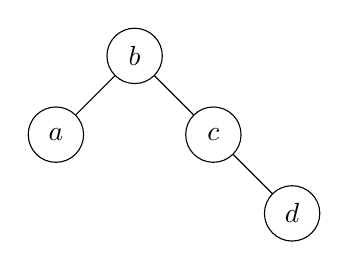
\begin{tikzpicture}
  [node/.style={circle,draw,minimum size=2em}]
  \node[node] (A) at (-1,-1) {$a$};
  \node[node] (B) at (0,0) {$b$};
  \node[node] (C) at (1,-1) {$c$};
  \node[node] (D) at (2,-2) {$d$};
  
  \draw (A) -- (B);
  \draw (B) -- (C);
  \draw (C) -- (D);
\end{tikzpicture}
\end{minipage}
\begin{minipage}[c]{0.3\textwidth}
\centering
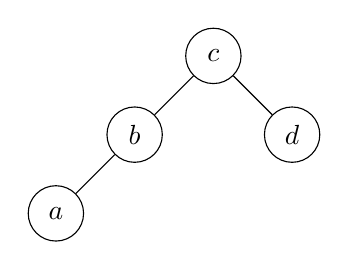
\begin{tikzpicture}
  [node/.style={circle,draw,minimum size=2em}]
  \node[node] (A) at (-2,-2) {$a$};
  \node[node] (B) at (-1,-1) {$b$};
  \node[node] (C) at (0,0) {$c$};
  \node[node] (D) at (1,-1) {$d$};
  
  \draw (A) -- (B);
  \draw (B) -- (C);
  \draw (C) -- (D);
\end{tikzpicture}
\end{minipage}
\caption{Tabela com o número de ocorrências por chave em uma sequência de entrada. À esquerda, árvore gerada pelo algoritmo guloso, com custo total 75, e à direita, árvore ótima, com custo total 65.}
\label{fig:caso-guloso-subotimo}
\end{figure}

\section{Algoritmo ótimo}

A análise da seção anterior nos leva a perceber que precisamos de uma conduta que considere tanto o número de ocorrências de cada nó quanto a estrutura da árvore em si. Um algoritmo para encontrar a ABB ótima foi desenvolvido por \cite{knuth}.

Primeiramente é preciso entender como a estrutura de uma árvore ótima está disposta. Consideremos que a árvore possui as chaves em um intervalo contínuo de 1 até $n$. 

Para uma árvore $T$ com chave $k$ na raiz ser ótima, a sua subárvore esquerda, contendo as chaves $1,\dots,k$, deve ser ótima e sua subárvore direita, contendo as chaves $k$+1$,\dots,n$, deve ser ótima também.

Isso pode ser provado da seguinte maneira. Seja $T$ uma árvore ótima para uma entrada $X$ com chave $k$ na raiz e seja $T'$ a sub-árvore de $k$ que não é ótima. Como $T'$ não é ótima, então existe uma árvore $T''$ ótima que também possui as mesmas chaves de $T'$, mas possui custo menor para os acessos de $X$. Assim, é possível trocar a sub-árvore $T'$ pela sub-árvore $T''$ em $T$ e encontramos uma árvore com custo menor que $T$. Como $T$ é uma árvore ótima, isso é uma contradição.

Assim, sabemos que para um intervalo $k_i, \ldots, k_j$ ($i \leq j$), a árvore ótima possui um nó com chave $k_r$ ($i \leq r \leq j$) como raiz e duas subárvores possivelmente vazias como filhas. A sub-árvore esquerda é uma árvore ótima que contém as chaves $k_i, \ldots, k_{r-1}$ e a sub-árvore direita é uma árvore ótima que contém as chaves $k_{r+1}, \ldots, k_j$.

Levando em consideração essa estrutura, dado um intervalo de chaves $k_i, \ldots, k_j$, o algoritmo ótimo precisa descobrir qual das chaves deve permanecer no nó raiz para minimizar o custo total.